\documentclass[1p]{elsarticle_modified}
%\bibliographystyle{elsarticle-num}

%\usepackage[colorlinks]{hyperref}
%\usepackage{abbrmath_seonhwa} %\Abb, \Ascr, \Acal ,\Abf, \Afrak
\usepackage{amsfonts}
\usepackage{amssymb}
\usepackage{amsmath}
\usepackage{amsthm}
\usepackage{scalefnt}
\usepackage{amsbsy}
\usepackage{kotex}
\usepackage{caption}
\usepackage{subfig}
\usepackage{color}
\usepackage{graphicx}
\usepackage{xcolor} %% white, black, red, green, blue, cyan, magenta, yellow
\usepackage{float}
\usepackage{setspace}
\usepackage{hyperref}

\usepackage{tikz}
\usetikzlibrary{arrows}

\usepackage{multirow}
\usepackage{array} % fixed length table
\usepackage{hhline}

%%%%%%%%%%%%%%%%%%%%%
\makeatletter
\renewcommand*\env@matrix[1][\arraystretch]{%
	\edef\arraystretch{#1}%
	\hskip -\arraycolsep
	\let\@ifnextchar\new@ifnextchar
	\array{*\c@MaxMatrixCols c}}
\makeatother %https://tex.stackexchange.com/questions/14071/how-can-i-increase-the-line-spacing-in-a-matrix
%%%%%%%%%%%%%%%

\usepackage[normalem]{ulem}

\newcommand{\msout}[1]{\ifmmode\text{\sout{\ensuremath{#1}}}\else\sout{#1}\fi}
%SOURCE: \msout is \stkout macro in https://tex.stackexchange.com/questions/20609/strikeout-in-math-mode

\newcommand{\cancel}[1]{
	\ifmmode
	{\color{red}\msout{#1}}
	\else
	{\color{red}\sout{#1}}
	\fi
}

\newcommand{\add}[1]{
	{\color{blue}\uwave{#1}}
}

\newcommand{\replace}[2]{
	\ifmmode
	{\color{red}\msout{#1}}{\color{blue}\uwave{#2}}
	\else
	{\color{red}\sout{#1}}{\color{blue}\uwave{#2}}
	\fi
}

\newcommand{\Sol}{\mathcal{S}} %segment
\newcommand{\D}{D} %diagram
\newcommand{\A}{\mathcal{A}} %arc


%%%%%%%%%%%%%%%%%%%%%%%%%%%%%5 test

\def\sl{\operatorname{\textup{SL}}(2,\Cbb)}
\def\psl{\operatorname{\textup{PSL}}(2,\Cbb)}
\def\quan{\mkern 1mu \triangleright \mkern 1mu}

\theoremstyle{definition}
\newtheorem{thm}{Theorem}[section]
\newtheorem{prop}[thm]{Proposition}
\newtheorem{lem}[thm]{Lemma}
\newtheorem{ques}[thm]{Question}
\newtheorem{cor}[thm]{Corollary}
\newtheorem{defn}[thm]{Definition}
\newtheorem{exam}[thm]{Example}
\newtheorem{rmk}[thm]{Remark}
\newtheorem{alg}[thm]{Algorithm}

\newcommand{\I}{\sqrt{-1}}
\begin{document}

%\begin{frontmatter}
%
%\title{Boundary parabolic representations of knots up to 8 crossings}
%
%%% Group authors per affiliation:
%\author{Yunhi Cho} 
%\address{Department of Mathematics, University of Seoul, Seoul, Korea}
%\ead{yhcho@uos.ac.kr}
%
%
%\author{Seonhwa Kim} %\fnref{s_kim}}
%\address{Center for Geometry and Physics, Institute for Basic Science, Pohang, 37673, Korea}
%\ead{ryeona17@ibs.re.kr}
%
%\author{Hyuk Kim}
%\address{Department of Mathematical Sciences, Seoul National University, Seoul 08826, Korea}
%\ead{hyukkim@snu.ac.kr}
%
%\author{Seokbeom Yoon}
%\address{Department of Mathematical Sciences, Seoul National University, Seoul, 08826,  Korea}
%\ead{sbyoon15@snu.ac.kr}
%
%\begin{abstract}
%We find all boundary parabolic representation of knots up to 8 crossings.
%
%\end{abstract}
%\begin{keyword}
%    \MSC[2010] 57M25 
%\end{keyword}
%
%\end{frontmatter}

%\linenumbers
%\tableofcontents
%
\newcommand\colored[1]{\textcolor{white}{\rule[-0.35ex]{0.8em}{1.4ex}}\kern-0.8em\color{red} #1}%
%\newcommand\colored[1]{\textcolor{white}{ #1}\kern-2.17ex	\textcolor{white}{ #1}\kern-1.81ex	\textcolor{white}{ #1}\kern-2.15ex\color{red}#1	}

{\Large $\underline{11n_{64}~(K11n_{64})}$}

\setlength{\tabcolsep}{10pt}
\renewcommand{\arraystretch}{1.6}
\vspace{1cm}\begin{tabular}{m{100pt}>{\centering\arraybackslash}m{274pt}}
\multirow{5}{120pt}{
	\centering
	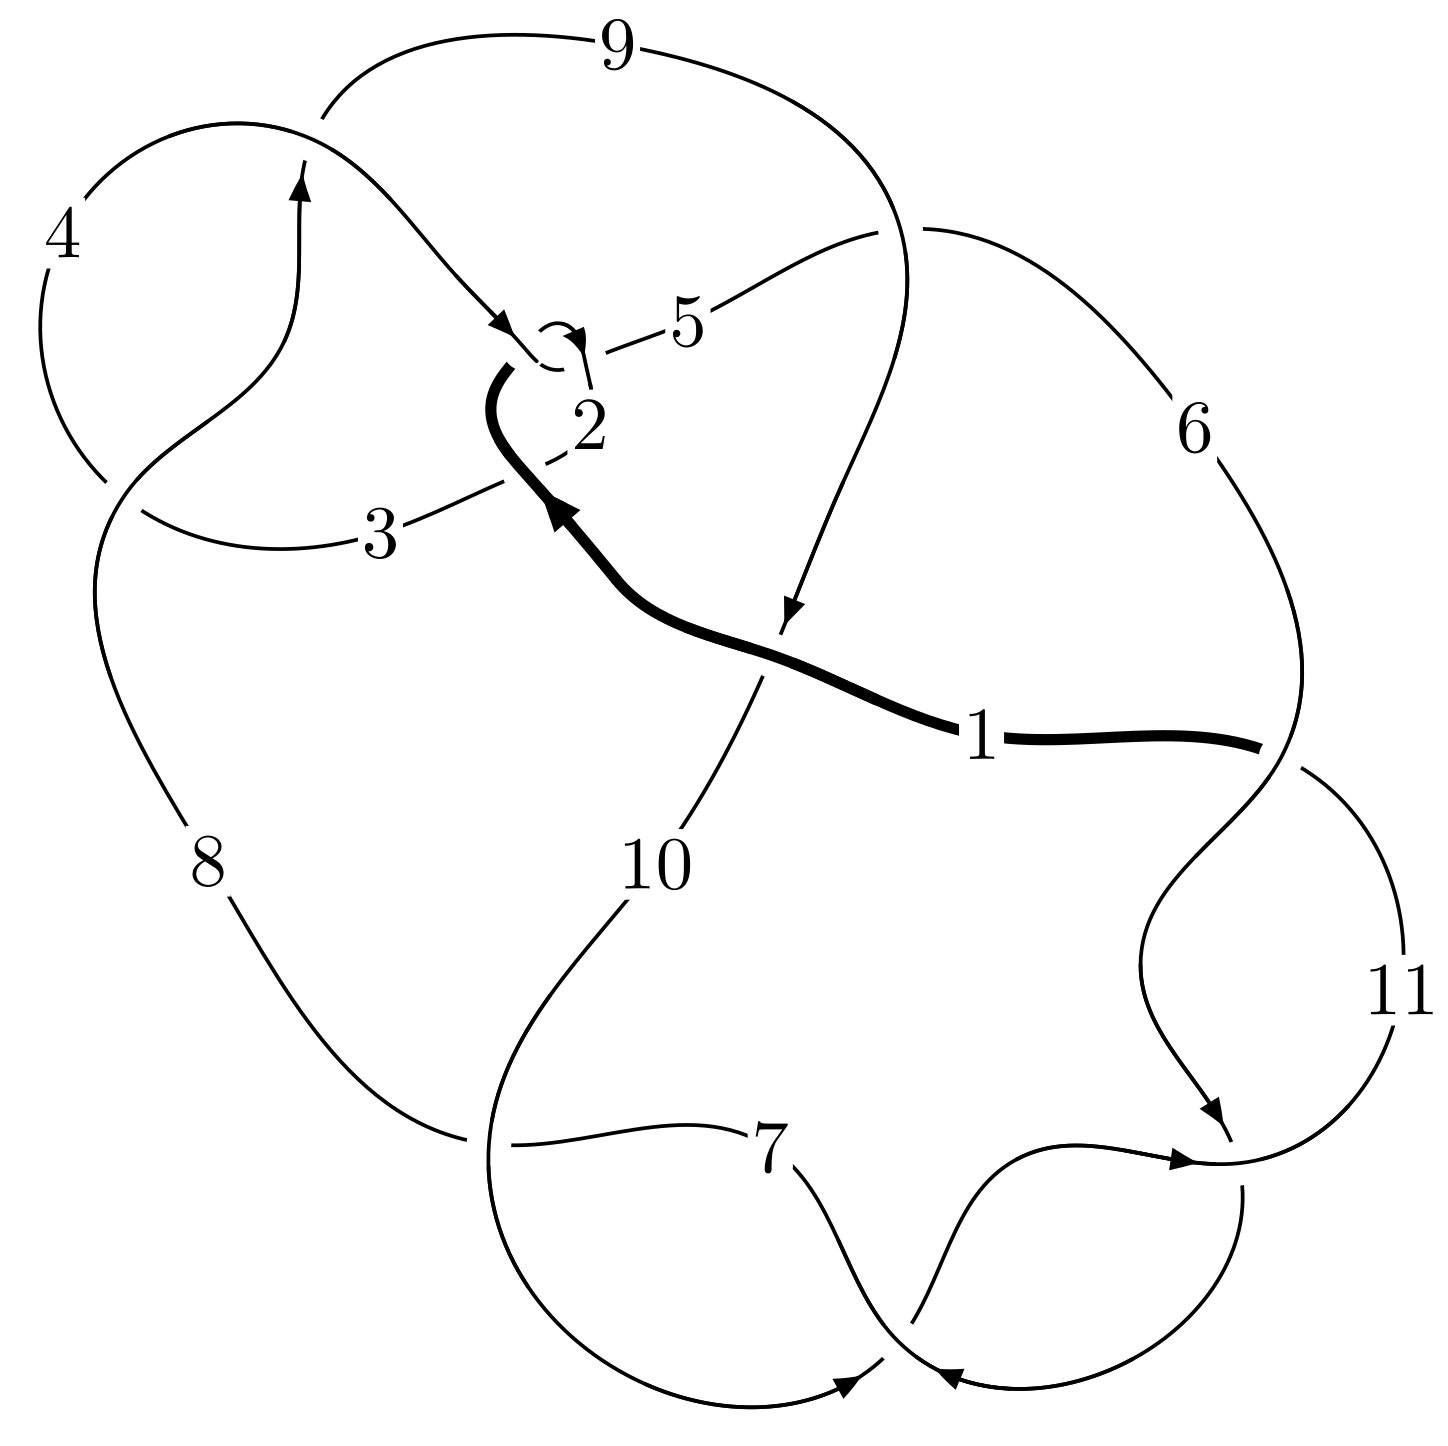
\includegraphics[width=112pt]{../../../GIT/diagram.site/Diagrams/png/680_11n_64.png}\\
\ \ \ A knot diagram\footnotemark}&
\allowdisplaybreaks
\textbf{Linearized knot diagam} \\
\cline{2-2}
 &
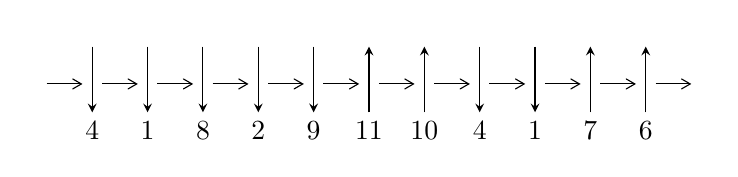
\begin{tikzpicture}[x=20pt, y=17pt]
	% nodes
	\node (C0) at (0, 0) {};
	\node (C1) at (1, 0) {};
	\node (C1U) at (1, +1) {};
	\node (C1D) at (1, -1) {4};

	\node (C2) at (2, 0) {};
	\node (C2U) at (2, +1) {};
	\node (C2D) at (2, -1) {1};

	\node (C3) at (3, 0) {};
	\node (C3U) at (3, +1) {};
	\node (C3D) at (3, -1) {8};

	\node (C4) at (4, 0) {};
	\node (C4U) at (4, +1) {};
	\node (C4D) at (4, -1) {2};

	\node (C5) at (5, 0) {};
	\node (C5U) at (5, +1) {};
	\node (C5D) at (5, -1) {9};

	\node (C6) at (6, 0) {};
	\node (C6U) at (6, +1) {};
	\node (C6D) at (6, -1) {11};

	\node (C7) at (7, 0) {};
	\node (C7U) at (7, +1) {};
	\node (C7D) at (7, -1) {10};

	\node (C8) at (8, 0) {};
	\node (C8U) at (8, +1) {};
	\node (C8D) at (8, -1) {4};

	\node (C9) at (9, 0) {};
	\node (C9U) at (9, +1) {};
	\node (C9D) at (9, -1) {1};

	\node (C10) at (10, 0) {};
	\node (C10U) at (10, +1) {};
	\node (C10D) at (10, -1) {7};

	\node (C11) at (11, 0) {};
	\node (C11U) at (11, +1) {};
	\node (C11D) at (11, -1) {6};
	\node (C12) at (12, 0) {};

	% arrows
	\draw[->,>={angle 60}]
	(C0) edge (C1) (C1) edge (C2) (C2) edge (C3) (C3) edge (C4) (C4) edge (C5) (C5) edge (C6) (C6) edge (C7) (C7) edge (C8) (C8) edge (C9) (C9) edge (C10) (C10) edge (C11) (C11) edge (C12) ;	\draw[->,>=stealth]
	(C1U) edge (C1D) (C2U) edge (C2D) (C3U) edge (C3D) (C4U) edge (C4D) (C5U) edge (C5D) (C6D) edge (C6U) (C7D) edge (C7U) (C8U) edge (C8D) (C9U) edge (C9D) (C10D) edge (C10U) (C11D) edge (C11U) ;
	\end{tikzpicture} \\
\hhline{~~} \\& 
\textbf{Solving Sequence} \\ \cline{2-2} 
 &
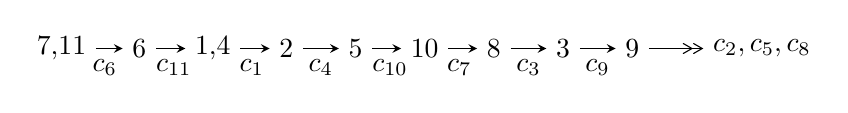
\begin{tikzpicture}[x=25pt, y=7pt]
	% node
	\node (A0) at (-1/8, 0) {7,11};
	\node (A1) at (1, 0) {6};
	\node (A2) at (33/16, 0) {1,4};
	\node (A3) at (25/8, 0) {2};
	\node (A4) at (33/8, 0) {5};
	\node (A5) at (41/8, 0) {10};
	\node (A6) at (49/8, 0) {8};
	\node (A7) at (57/8, 0) {3};
	\node (A8) at (65/8, 0) {9};
	\node (C1) at (1/2, -1) {$c_{6}$};
	\node (C2) at (3/2, -1) {$c_{11}$};
	\node (C3) at (21/8, -1) {$c_{1}$};
	\node (C4) at (29/8, -1) {$c_{4}$};
	\node (C5) at (37/8, -1) {$c_{10}$};
	\node (C6) at (45/8, -1) {$c_{7}$};
	\node (C7) at (53/8, -1) {$c_{3}$};
	\node (C8) at (61/8, -1) {$c_{9}$};
	\node (A9) at (10, 0) {$c_{2},c_{5},c_{8}$};

	% edge
	\draw[->,>=stealth]	
	(A0) edge (A1) (A1) edge (A2) (A2) edge (A3) (A3) edge (A4) (A4) edge (A5) (A5) edge (A6) (A6) edge (A7) (A7) edge (A8) ;
	\draw[->>,>={angle 60}]	
	(A8) edge (A9);
\end{tikzpicture} \\ 

\end{tabular} \\

\footnotetext{
The image of knot diagram is generated by the software ``\textbf{Draw programme}" developed by Andrew Bartholomew(\url{http://www.layer8.co.uk/maths/draw/index.htm\#Running-draw}), where we modified some parts for our purpose(\url{https://github.com/CATsTAILs/LinksPainter}).
}\phantom \\ \newline 
\centering \textbf{Ideals for irreducible components\footnotemark of $X_{\text{par}}$} 
 
\begin{align*}
I^u_{1}&=\langle 
u^{11}-2 u^{10}+8 u^9-12 u^8+22 u^7-23 u^6+24 u^5-15 u^4+9 u^3-4 u^2+b+2 u-1,\\
\phantom{I^u_{1}}&\phantom{= \langle  }- u^{13}+2 u^{12}-11 u^{11}+18 u^{10}-45 u^9+58 u^8-84 u^7+79 u^6-70 u^5+43 u^4-23 u^3+14 u^2+a-5 u+3,\\
\phantom{I^u_{1}}&\phantom{= \langle  }u^{14}-2 u^{13}+11 u^{12}-18 u^{11}+46 u^{10}-60 u^9+91 u^8-90 u^7+86 u^6-61 u^5+36 u^4-22 u^3+8 u^2-5 u+1\rangle \\
I^u_{2}&=\langle 
u^2+b+u+1,\;- u^3- u^2+a-3 u-1,\;u^4+u^3+3 u^2+2 u+1\rangle \\
\\
\end{align*}
\raggedright * 2 irreducible components of $\dim_{\mathbb{C}}=0$, with total 18 representations.\\
\footnotetext{All coefficients of polynomials are rational numbers. But the coefficients are sometimes approximated in decimal forms when there is not enough margin.}
\newpage
\renewcommand{\arraystretch}{1}
\centering \section*{I. $I^u_{1}= \langle u^{11}-2 u^{10}+\cdots+b-1,\;- u^{13}+2 u^{12}+\cdots+a+3,\;u^{14}-2 u^{13}+\cdots-5 u+1 \rangle$}
\flushleft \textbf{(i) Arc colorings}\\
\begin{tabular}{m{7pt} m{180pt} m{7pt} m{180pt} }
\flushright $a_{7}=$&$\begin{pmatrix}1\\0\end{pmatrix}$ \\
\flushright $a_{11}=$&$\begin{pmatrix}0\\u\end{pmatrix}$ \\
\flushright $a_{6}=$&$\begin{pmatrix}1\\u^2\end{pmatrix}$ \\
\flushright $a_{1}=$&$\begin{pmatrix}u\\u^3+u\end{pmatrix}$ \\
\flushright $a_{4}=$&$\begin{pmatrix}u^{13}-2 u^{12}+\cdots+5 u-3\\- u^{11}+2 u^{10}+\cdots-2 u+1\end{pmatrix}$ \\
\flushright $a_{2}=$&$\begin{pmatrix}u^{13}-2 u^{12}+\cdots+4 u-2\\u^{12}-2 u^{11}+\cdots-2 u+1\end{pmatrix}$ \\
\flushright $a_{5}=$&$\begin{pmatrix}u^{10}+5 u^8+6 u^6- u^4- u^2-1\\u^{12}+6 u^{10}+12 u^8+10 u^6+5 u^4\end{pmatrix}$ \\
\flushright $a_{10}=$&$\begin{pmatrix}- u\\u\end{pmatrix}$ \\
\flushright $a_{8}=$&$\begin{pmatrix}u^2+1\\- u^2\end{pmatrix}$ \\
\flushright $a_{3}=$&$\begin{pmatrix}u^{13}-2 u^{12}+\cdots+3 u-2\\- u^{13}+2 u^{12}+\cdots-3 u+1\end{pmatrix}$ \\
\flushright $a_{9}=$&$\begin{pmatrix}u^5+2 u^3- u\\u^7+3 u^5+2 u^3+u\end{pmatrix}$\\ \flushright $a_{9}=$&$\begin{pmatrix}u^5+2 u^3- u\\u^7+3 u^5+2 u^3+u\end{pmatrix}$\\&\end{tabular}
\flushleft \textbf{(ii) Obstruction class $= -1$}\\~\\
\flushleft \textbf{(iii) Cusp Shapes $= - u^{13}+2 u^{12}-11 u^{11}+17 u^{10}-42 u^9+48 u^8-62 u^7+44 u^6-17 u^5-7 u^4+23 u^3-11 u^2+6 u-9$}\\~\\
\newpage\renewcommand{\arraystretch}{1}
\flushleft \textbf{(iv) u-Polynomials at the component}\newline \\
\begin{tabular}{m{50pt}|m{274pt}}
Crossings & \hspace{64pt}u-Polynomials at each crossing \\
\hline $$\begin{aligned}c_{1},c_{4}\end{aligned}$$&$\begin{aligned}
&u^{14}-5 u^{13}+\cdots+7 u-1
\end{aligned}$\\
\hline $$\begin{aligned}c_{2}\end{aligned}$$&$\begin{aligned}
&u^{14}+23 u^{13}+\cdots+3 u+1
\end{aligned}$\\
\hline $$\begin{aligned}c_{3},c_{8}\end{aligned}$$&$\begin{aligned}
&u^{14}- u^{13}+\cdots-24 u-16
\end{aligned}$\\
\hline $$\begin{aligned}c_{5}\end{aligned}$$&$\begin{aligned}
&u^{14}+2 u^{13}+\cdots+3 u+1
\end{aligned}$\\
\hline $$\begin{aligned}c_{6},c_{7},c_{10}\\c_{11}\end{aligned}$$&$\begin{aligned}
&u^{14}+2 u^{13}+\cdots+5 u+1
\end{aligned}$\\
\hline $$\begin{aligned}c_{9}\end{aligned}$$&$\begin{aligned}
&u^{14}-6 u^{13}+\cdots-117 u+19
\end{aligned}$\\
\hline
\end{tabular}\\~\\
\newpage\renewcommand{\arraystretch}{1}
\flushleft \textbf{(v) Riley Polynomials at the component}\newline \\
\begin{tabular}{m{50pt}|m{274pt}}
Crossings & \hspace{64pt}Riley Polynomials at each crossing \\
\hline $$\begin{aligned}c_{1},c_{4}\end{aligned}$$&$\begin{aligned}
&y^{14}-23 y^{13}+\cdots-3 y+1
\end{aligned}$\\
\hline $$\begin{aligned}c_{2}\end{aligned}$$&$\begin{aligned}
&y^{14}-59 y^{13}+\cdots+681 y+1
\end{aligned}$\\
\hline $$\begin{aligned}c_{3},c_{8}\end{aligned}$$&$\begin{aligned}
&y^{14}-27 y^{13}+\cdots+960 y+256
\end{aligned}$\\
\hline $$\begin{aligned}c_{5}\end{aligned}$$&$\begin{aligned}
&y^{14}-30 y^{13}+\cdots-9 y+1
\end{aligned}$\\
\hline $$\begin{aligned}c_{6},c_{7},c_{10}\\c_{11}\end{aligned}$$&$\begin{aligned}
&y^{14}+18 y^{13}+\cdots-9 y+1
\end{aligned}$\\
\hline $$\begin{aligned}c_{9}\end{aligned}$$&$\begin{aligned}
&y^{14}-18 y^{13}+\cdots-22277 y+361
\end{aligned}$\\
\hline
\end{tabular}\\~\\
\newpage\flushleft \textbf{(vi) Complex Volumes and Cusp Shapes}
$$\begin{array}{c|c|c}  
\text{Solutions to }I^u_{1}& \I (\text{vol} + \sqrt{-1}CS) & \text{Cusp shape}\\
 \hline 
\begin{aligned}
u &= \phantom{-}0.550866 + 0.900632 I \\
a &= -1.08064 - 1.46517 I \\
b &= \phantom{-}0.098170 - 0.182990 I\end{aligned}
 & -14.5979 + 4.4309 I & -8.77759 - 3.45380 I \\ \hline\begin{aligned}
u &= \phantom{-}0.550866 - 0.900632 I \\
a &= -1.08064 + 1.46517 I \\
b &= \phantom{-}0.098170 + 0.182990 I\end{aligned}
 & -14.5979 - 4.4309 I & -8.77759 + 3.45380 I \\ \hline\begin{aligned}
u &= \phantom{-}0.131850 + 0.795140 I \\
a &= \phantom{-}1.42680 + 0.95287 I \\
b &= \phantom{-}0.002648 - 0.749310 I\end{aligned}
 & -3.41989 + 1.31906 I & -10.67824 - 1.83447 I \\ \hline\begin{aligned}
u &= \phantom{-}0.131850 - 0.795140 I \\
a &= \phantom{-}1.42680 - 0.95287 I \\
b &= \phantom{-}0.002648 + 0.749310 I\end{aligned}
 & -3.41989 - 1.31906 I & -10.67824 + 1.83447 I \\ \hline\begin{aligned}
u &= \phantom{-}0.778815\phantom{ +0.000000I} \\
a &= \phantom{-}0.532114\phantom{ +0.000000I} \\
b &= -1.55087\phantom{ +0.000000I}\end{aligned}
 & -11.8742\phantom{ +0.000000I} & -5.71440\phantom{ +0.000000I} \\ \hline\begin{aligned}
u &= -0.310969 + 0.512101 I \\
a &= -0.546661 + 0.069487 I \\
b &= -0.054284 + 0.327429 I\end{aligned}
 & -0.044354 - 1.170560 I & -0.70219 + 5.58030 I \\ \hline\begin{aligned}
u &= -0.310969 - 0.512101 I \\
a &= -0.546661 - 0.069487 I \\
b &= -0.054284 - 0.327429 I\end{aligned}
 & -0.044354 + 1.170560 I & -0.70219 - 5.58030 I \\ \hline\begin{aligned}
u &= -0.07909 + 1.57522 I \\
a &= -0.593424 + 0.223836 I \\
b &= \phantom{-}1.203460 + 0.007835 I\end{aligned}
 & -7.25996 - 2.49887 I & -4.67922 + 1.75896 I \\ \hline\begin{aligned}
u &= -0.07909 - 1.57522 I \\
a &= -0.593424 - 0.223836 I \\
b &= \phantom{-}1.203460 - 0.007835 I\end{aligned}
 & -7.25996 + 2.49887 I & -4.67922 - 1.75896 I \\ \hline\begin{aligned}
u &= \phantom{-}0.03110 + 1.66209 I \\
a &= \phantom{-}1.73343 + 0.06583 I \\
b &= -3.48457 - 0.73242 I\end{aligned}
 & -12.09880 + 1.91262 I & -10.51406 - 1.13289 I\\
 \hline 
 \end{array}$$\newpage$$\begin{array}{c|c|c}  
\text{Solutions to }I^u_{1}& \I (\text{vol} + \sqrt{-1}CS) & \text{Cusp shape}\\
 \hline 
\begin{aligned}
u &= \phantom{-}0.03110 - 1.66209 I \\
a &= \phantom{-}1.73343 - 0.06583 I \\
b &= -3.48457 + 0.73242 I\end{aligned}
 & -12.09880 - 1.91262 I & -10.51406 + 1.13289 I \\ \hline\begin{aligned}
u &= \phantom{-}0.16129 + 1.68407 I \\
a &= -2.01585 - 0.88397 I \\
b &= \phantom{-}4.18614 + 1.67352 I\end{aligned}
 & \phantom{-}15.9841 + 7.2397 I & -10.36154 - 2.69654 I \\ \hline\begin{aligned}
u &= \phantom{-}0.16129 - 1.68407 I \\
a &= -2.01585 + 0.88397 I \\
b &= \phantom{-}4.18614 - 1.67352 I\end{aligned}
 & \phantom{-}15.9841 - 7.2397 I & -10.36154 + 2.69654 I \\ \hline\begin{aligned}
u &= \phantom{-}0.251089\phantom{ +0.000000I} \\
a &= -2.37942\phantom{ +0.000000I} \\
b &= \phantom{-}0.647742\phantom{ +0.000000I}\end{aligned}
 & -1.17986\phantom{ +0.000000I} & -7.85990\phantom{ +0.000000I}\\
 \hline 
 \end{array}$$\newpage\newpage\renewcommand{\arraystretch}{1}
\centering \section*{II. $I^u_{2}= \langle u^2+b+u+1,\;- u^3- u^2+a-3 u-1,\;u^4+u^3+3 u^2+2 u+1 \rangle$}
\flushleft \textbf{(i) Arc colorings}\\
\begin{tabular}{m{7pt} m{180pt} m{7pt} m{180pt} }
\flushright $a_{7}=$&$\begin{pmatrix}1\\0\end{pmatrix}$ \\
\flushright $a_{11}=$&$\begin{pmatrix}0\\u\end{pmatrix}$ \\
\flushright $a_{6}=$&$\begin{pmatrix}1\\u^2\end{pmatrix}$ \\
\flushright $a_{1}=$&$\begin{pmatrix}u\\u^3+u\end{pmatrix}$ \\
\flushright $a_{4}=$&$\begin{pmatrix}u^3+u^2+3 u+1\\- u^2- u-1\end{pmatrix}$ \\
\flushright $a_{2}=$&$\begin{pmatrix}u^3+u^2+4 u+1\\u^3- u^2-1\end{pmatrix}$ \\
\flushright $a_{5}=$&$\begin{pmatrix}- u\\- u^3- u\end{pmatrix}$ \\
\flushright $a_{10}=$&$\begin{pmatrix}- u\\u\end{pmatrix}$ \\
\flushright $a_{8}=$&$\begin{pmatrix}u^2+1\\- u^2\end{pmatrix}$ \\
\flushright $a_{3}=$&$\begin{pmatrix}u^3+u^2+3 u+1\\- u^2- u-1\end{pmatrix}$ \\
\flushright $a_{9}=$&$\begin{pmatrix}u^2+1\\- u^2\end{pmatrix}$\\ \flushright $a_{9}=$&$\begin{pmatrix}u^2+1\\- u^2\end{pmatrix}$\\&\end{tabular}
\flushleft \textbf{(ii) Obstruction class $= 1$}\\~\\
\flushleft \textbf{(iii) Cusp Shapes $= 3 u^3+3 u^2+10 u-4$}\\~\\
\newpage\renewcommand{\arraystretch}{1}
\flushleft \textbf{(iv) u-Polynomials at the component}\newline \\
\begin{tabular}{m{50pt}|m{274pt}}
Crossings & \hspace{64pt}u-Polynomials at each crossing \\
\hline $$\begin{aligned}c_{1}\end{aligned}$$&$\begin{aligned}
&(u-1)^4
\end{aligned}$\\
\hline $$\begin{aligned}c_{2},c_{4}\end{aligned}$$&$\begin{aligned}
&(u+1)^4
\end{aligned}$\\
\hline $$\begin{aligned}c_{3},c_{8}\end{aligned}$$&$\begin{aligned}
&u^4
\end{aligned}$\\
\hline $$\begin{aligned}c_{5},c_{9}\end{aligned}$$&$\begin{aligned}
&u^4+u^3+u^2+1
\end{aligned}$\\
\hline $$\begin{aligned}c_{6},c_{7}\end{aligned}$$&$\begin{aligned}
&u^4+u^3+3 u^2+2 u+1
\end{aligned}$\\
\hline $$\begin{aligned}c_{10},c_{11}\end{aligned}$$&$\begin{aligned}
&u^4- u^3+3 u^2-2 u+1
\end{aligned}$\\
\hline
\end{tabular}\\~\\
\newpage\renewcommand{\arraystretch}{1}
\flushleft \textbf{(v) Riley Polynomials at the component}\newline \\
\begin{tabular}{m{50pt}|m{274pt}}
Crossings & \hspace{64pt}Riley Polynomials at each crossing \\
\hline $$\begin{aligned}c_{1},c_{2},c_{4}\end{aligned}$$&$\begin{aligned}
&(y-1)^4
\end{aligned}$\\
\hline $$\begin{aligned}c_{3},c_{8}\end{aligned}$$&$\begin{aligned}
&y^4
\end{aligned}$\\
\hline $$\begin{aligned}c_{5},c_{9}\end{aligned}$$&$\begin{aligned}
&y^4+y^3+3 y^2+2 y+1
\end{aligned}$\\
\hline $$\begin{aligned}c_{6},c_{7},c_{10}\\c_{11}\end{aligned}$$&$\begin{aligned}
&y^4+5 y^3+7 y^2+2 y+1
\end{aligned}$\\
\hline
\end{tabular}\\~\\
\newpage\flushleft \textbf{(vi) Complex Volumes and Cusp Shapes}
$$\begin{array}{c|c|c}  
\text{Solutions to }I^u_{2}& \I (\text{vol} + \sqrt{-1}CS) & \text{Cusp shape}\\
 \hline 
\begin{aligned}
u &= -0.395123 + 0.506844 I \\
a &= -0.043315 + 1.227190 I \\
b &= -0.504108 - 0.106312 I\end{aligned}
 & -1.43393 - 1.41510 I & -7.52507 + 4.18840 I \\ \hline\begin{aligned}
u &= -0.395123 - 0.506844 I \\
a &= -0.043315 - 1.227190 I \\
b &= -0.504108 + 0.106312 I\end{aligned}
 & -1.43393 + 1.41510 I & -7.52507 - 4.18840 I \\ \hline\begin{aligned}
u &= -0.10488 + 1.55249 I \\
a &= -0.956685 + 0.641200 I \\
b &= \phantom{-}1.50411 - 1.22685 I\end{aligned}
 & -8.43568 - 3.16396 I & -9.97493 + 3.47609 I \\ \hline\begin{aligned}
u &= -0.10488 - 1.55249 I \\
a &= -0.956685 - 0.641200 I \\
b &= \phantom{-}1.50411 + 1.22685 I\end{aligned}
 & -8.43568 + 3.16396 I & -9.97493 - 3.47609 I\\
 \hline 
 \end{array}$$\newpage
\newpage\renewcommand{\arraystretch}{1}
\centering \section*{ III. u-Polynomials}
\begin{tabular}{m{50pt}|m{274pt}}
Crossings & \hspace{64pt}u-Polynomials at each crossing \\
\hline $$\begin{aligned}c_{1}\end{aligned}$$&$\begin{aligned}
&((u-1)^4)(u^{14}-5 u^{13}+\cdots+7 u-1)
\end{aligned}$\\
\hline $$\begin{aligned}c_{2}\end{aligned}$$&$\begin{aligned}
&((u+1)^4)(u^{14}+23 u^{13}+\cdots+3 u+1)
\end{aligned}$\\
\hline $$\begin{aligned}c_{3},c_{8}\end{aligned}$$&$\begin{aligned}
&u^4(u^{14}- u^{13}+\cdots-24 u-16)
\end{aligned}$\\
\hline $$\begin{aligned}c_{4}\end{aligned}$$&$\begin{aligned}
&((u+1)^4)(u^{14}-5 u^{13}+\cdots+7 u-1)
\end{aligned}$\\
\hline $$\begin{aligned}c_{5}\end{aligned}$$&$\begin{aligned}
&(u^4+u^3+u^2+1)(u^{14}+2 u^{13}+\cdots+3 u+1)
\end{aligned}$\\
\hline $$\begin{aligned}c_{6},c_{7}\end{aligned}$$&$\begin{aligned}
&(u^4+u^3+3 u^2+2 u+1)(u^{14}+2 u^{13}+\cdots+5 u+1)
\end{aligned}$\\
\hline $$\begin{aligned}c_{9}\end{aligned}$$&$\begin{aligned}
&(u^4+u^3+u^2+1)(u^{14}-6 u^{13}+\cdots-117 u+19)
\end{aligned}$\\
\hline $$\begin{aligned}c_{10},c_{11}\end{aligned}$$&$\begin{aligned}
&(u^4- u^3+3 u^2-2 u+1)(u^{14}+2 u^{13}+\cdots+5 u+1)
\end{aligned}$\\
\hline
\end{tabular}\newpage\renewcommand{\arraystretch}{1}
\centering \section*{ IV. Riley Polynomials}
\begin{tabular}{m{50pt}|m{274pt}}
Crossings & \hspace{64pt}Riley Polynomials at each crossing \\
\hline $$\begin{aligned}c_{1},c_{4}\end{aligned}$$&$\begin{aligned}
&((y-1)^4)(y^{14}-23 y^{13}+\cdots-3 y+1)
\end{aligned}$\\
\hline $$\begin{aligned}c_{2}\end{aligned}$$&$\begin{aligned}
&((y-1)^4)(y^{14}-59 y^{13}+\cdots+681 y+1)
\end{aligned}$\\
\hline $$\begin{aligned}c_{3},c_{8}\end{aligned}$$&$\begin{aligned}
&y^4(y^{14}-27 y^{13}+\cdots+960 y+256)
\end{aligned}$\\
\hline $$\begin{aligned}c_{5}\end{aligned}$$&$\begin{aligned}
&(y^4+y^3+3 y^2+2 y+1)(y^{14}-30 y^{13}+\cdots-9 y+1)
\end{aligned}$\\
\hline $$\begin{aligned}c_{6},c_{7},c_{10}\\c_{11}\end{aligned}$$&$\begin{aligned}
&(y^4+5 y^3+7 y^2+2 y+1)(y^{14}+18 y^{13}+\cdots-9 y+1)
\end{aligned}$\\
\hline $$\begin{aligned}c_{9}\end{aligned}$$&$\begin{aligned}
&(y^4+y^3+3 y^2+2 y+1)(y^{14}-18 y^{13}+\cdots-22277 y+361)
\end{aligned}$\\
\hline
\end{tabular}
\vskip 2pc
\end{document}